\section{Preliminaries}

The User Space component is a server process that provides the web service. Its main tasks are to mediate the services of the translation memory and to reflect all the users' GUI activity and make the user's work persistent on the server and available always in the same state they finished their work.

The User Space is a Java Servlet which is run using the \emph{Jetty WebServer}. All of the User Space code is implemented in Java. It uses the \emph{Hibernate} object-relational mapping library. The same \emph{PostgreSQL} database as in the TM Core is used. The in-memory \emph{hsqldb} database is used for unit testing.

Because the TM Core is a separate module, it is also linked as a dependency to the User Space, but they run together as one process in one Java Virtual Machine. Their communication is done by invoking the core methods returning objects of the shared classes.

\section{Architecture}

To make the whole project as clear as possible, we try to use as much as possible from the shared classes and avoid using the User Space specific classes. If some additional functionality is required and cannot be incorporated into the shared classes, mostly the database and core calls, we wrap the shared classes into distinct User Space classes.

The server class which processes the calls on the first level contains the {\it Session} objects. These objects process the calls with association to the particular logged in users. These two classes are not a part of the set of shared classes.

The session class contains an object representing the user (a wrapper for the shared class). A hash table of active documents is there to access  them quickly. Both the document objects and translation result objects (which collect the source chunk, translation suggestion and the actual user's translation) are wrappers for the shared classes. However, the inner shared objects are used for communication with other components.

The more basic level than the translation result uses exactly the shared classes structure.

\section{Functionality Overview}

The User Space services are available via the RPC calls from the client side. While running the server, there exist one instance of the server class. The main task of the sever class is to process the calls from the clients -- which in fact means pass the calls further to the particular sessions and manage the sessions themselves. There is a method for every single operation that is possible to happen in the client.

After a user logs in, a Session object is created. It contains a unique session ID the client uses for authentication of its calls. A session object contains information about the user -- the user's settings and a set of the documents owned by the user available via the User object, and a hash table of documents which are currently in use with loaded chunks. When the user is logged in all of the calls are processed in the session class.

Until the user does not explicitly requests a document, only basic information about the document remains loaded into memory (basic facts about the movie, such as the time of the last changes of the document). Only if the user opens the document for editing or requests the export of the subtitle file, all the document chunks with the translation suggestions and already finished user translations are loaded. However, if the list of owned documents is queried, empty documents arrive to the client no matter if the documents are loaded in the User Space.

There is also a thread running in the server that checks how long the sessions are opened without any user actions. If this time exceeds the predefined session time out limit, either a short limit for common sessions or a long limit for permanent sessions, the session is terminated. Another situations when a session is terminated is when the user logs in although he already owns a session or explicitly logs out. When a session ends, basic information about the session is written to the database (user, start time, end time) to enable us to compute statistics about the usage of the application later.

\begin{figure}
\begin{center}
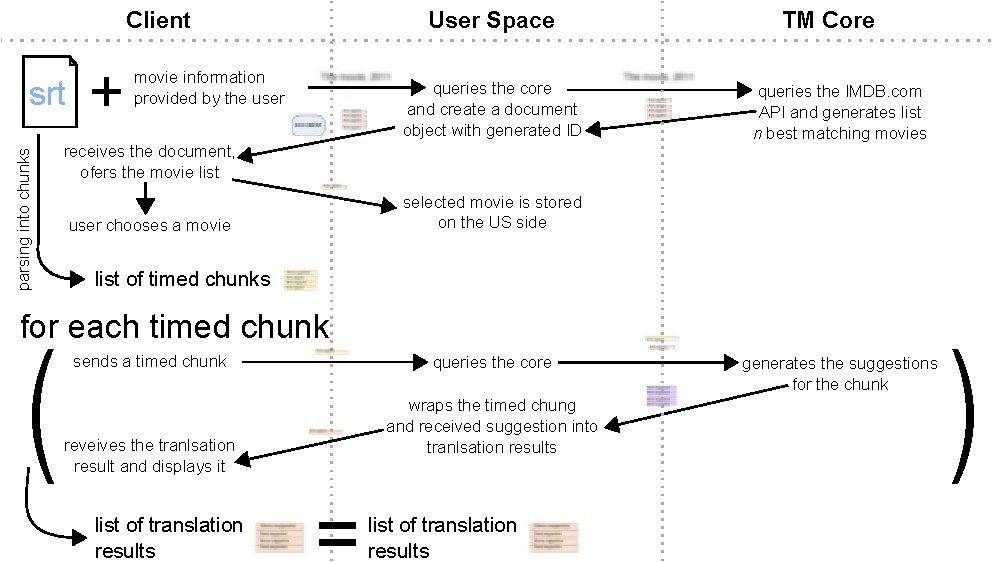
\includegraphics{figures/creating_document.pdf}
\end{center}
\caption{Structure of component communication during a new document creation}
\end{figure}

When a new document is created, the User Space receives basic information about the movie or TV show first. Based on that, it creates a Document object and saves it to the database immediately to receive a unique database ID which is then used as a document identifier in all other calls. The core is called at this moment to provide a list of possible movies with matching title and year of production together with genre tags obtained from the Freebase knowledge base. The user is then supposed to choose one or none of the suggested movies. This information is used by the User Space the moment the core is queried for the translation suggestions.

When a new document is created, the client application starts to send batches of chunks which are supposed to be translated. When the User Space receives such a call, it queries the TM Core for the translation suggestion and adds the chunks to the list of chunks which the appropriate document consists of. Once the suggestions are generated, they are sent to the GUI and the User Space does not persist them in any way. One reason to possibly keep the suggestions in memory or in the database is to avoid regenerating them. However, we decided that the cost of regenerating the suggestions is smaller than the cost of additionally storing suggestions in memory or in the database, which would increase the memory requirement significantly. When the client queries saved translation results, it will receive them without translation suggestions. For each untranslated chunk in the document, suggestions are generated and sent to the GUI on demand (see the GUI documentation in Section~\ref{sec:guiDocTrans}).

User Space also provides feedback to the translation memory. A list of new translations the users have produced can be generated together with information on which translation pair they used for post-editing is provided to the Data Import module which adds the new translation to the translation memory and use the data also for training the scoring of the suggestions (see Section~\ref{sec:ranking} in the Core documentation).

Export of the subtitle files is also solved in the User Space. It is described in more detail in section \ref{sec:export}.

\section{Implementation Details}
\subsection{Data Types Overview}

The User Space uses the shared classes used throughout the application or wrappers of such classes. A brief overview of the used classes and their role in the User Space follows. We use the abbreviation US to the refer the User Space in the following sections.

\begin{itemize}
\item {\tt FilmtitBackendServer}  -- The class is the Java Servlet whose public methods are invoked by the RPC calls. Its main task is to mediate the calls to concrete opened sessions and take care of users login. A thread checking if there is a sessions without activity for a long time and terminating the non-active sessions is run in the server class.

\item {\tt Session} -- The class represents a running session. There is exactly one session object for one logged in user, it is the Session class which processes the client calls. It contains hash tables of actively edited documents to make them quickly accessible by their IDs. During the existence of a session object, all the client-side operations are stored in memory and saved immediately to the database. When the session ends -- either by the user logging out or by exceeding the maximum time without a user action -- a record about the session is stored to database (id of the user that owned the session, its start time and end time). This is intended as an activity log from which further statistics can be inferred.

\item {\tt USUser} -- This class is a wrapper of the shared User class. During the existence of the session, it is used as a provider of the documents owned by the user. It is also used for storing the settings of the user. In contrast to the shared class, a set of documents which has been left opened when the last user's session was terminated is also stored in the class. This is used at the time a new session is created.

\item {\tt USDocument} -- The class is a wrapper of the shared {\tt Document} class. A {\tt USDocument} object represents a subtitle file with additional information about the movie it belongs to. Its content is supposed to be a mirror image of the Document object on the client side. It contains a list of Translation Results representing the actual subtitle chunks if the document is loaded to be edited. It is not connected to the translation results by the database mapping to make it easy to send a list of the user's documents without the actual content.

\item {\tt USTranslationResult} -- This class is a wrapper for the shared {\tt TranlsationResult} class. The class congregates the original subtitle chunk, its timing, the translations suggested by the translation memory and the result of the user activity (the users' translations, which translation suggestion they chose). It is the class where the actual translation is performed. Although a user can delete the document, all the translation results are kept in the database to provide feedback to the translation memory.

\item {\tt Emailer} -- A class used for sending email from the application. It is used for confirmation of user registration and also when the user forgets his password and requires sending a new one via email.

\end{itemize}

There are also two third-party classes included in the User Space source code. It is the {\tt IdGenerator} class which generates session ids (distributed under the {\it Apache License, Version 2.0}) and the {\tt BCrypt} class which ensures hashing the passwords before we store them in the database (distributed under {\it BSD licence}).

The {\tt SubtitleDownloadServlet} class responsible for exporting the subtitle files is described in Section~\ref{sec:export}. Details concerning the user registration, login and using open ID are discussed in more detail is Section~\ref{subsec:simple_login} in the GUI chapter. Details about handling the communication with the client are covered in Section~\ref{sec:communication} of the GUI chapter.

\subsection{Database Mapping}
\label{subsec:database_mapping}

As mentioned before, the User Space mirrors all the client's operations and makes them persistent on the server side. The persistence is ensured by saving the data to the database. The are a number of sophisticated tools for the JVM to ensure data persistence, e.g.\ the \emph{Java Persistence API} framework or some frameworks working on the higher level of abstraction, such as \emph{Spring Data Framework}. Since only very basic database operations are required during the operation of the User Space -- loading and saving of the raw Java object -- only a object relational mapping library is used, namely \emph{Hibernate}. The structure of the database being mapped is displayed in Figure~\ref{fig:em_of_us}.

User Space shares the mapping of the media source class and uses a class extended from the core class to manage the database transactions.

The mapping reflects the data properties of classes. If the class is a wrapper of a shared class, the getters and setters of the properties are bound to the wrapped objects properties.

As mentioned before, the mapping of {\tt USDocument} does not include the list of Translation Results the document contains in order to be able to send the documents both with and without the translation results. It would also be possible to use lazy Hibernate collection mappings, but it would cause problems at the time the object are serialized.

\begin{figure}
\begin{center}
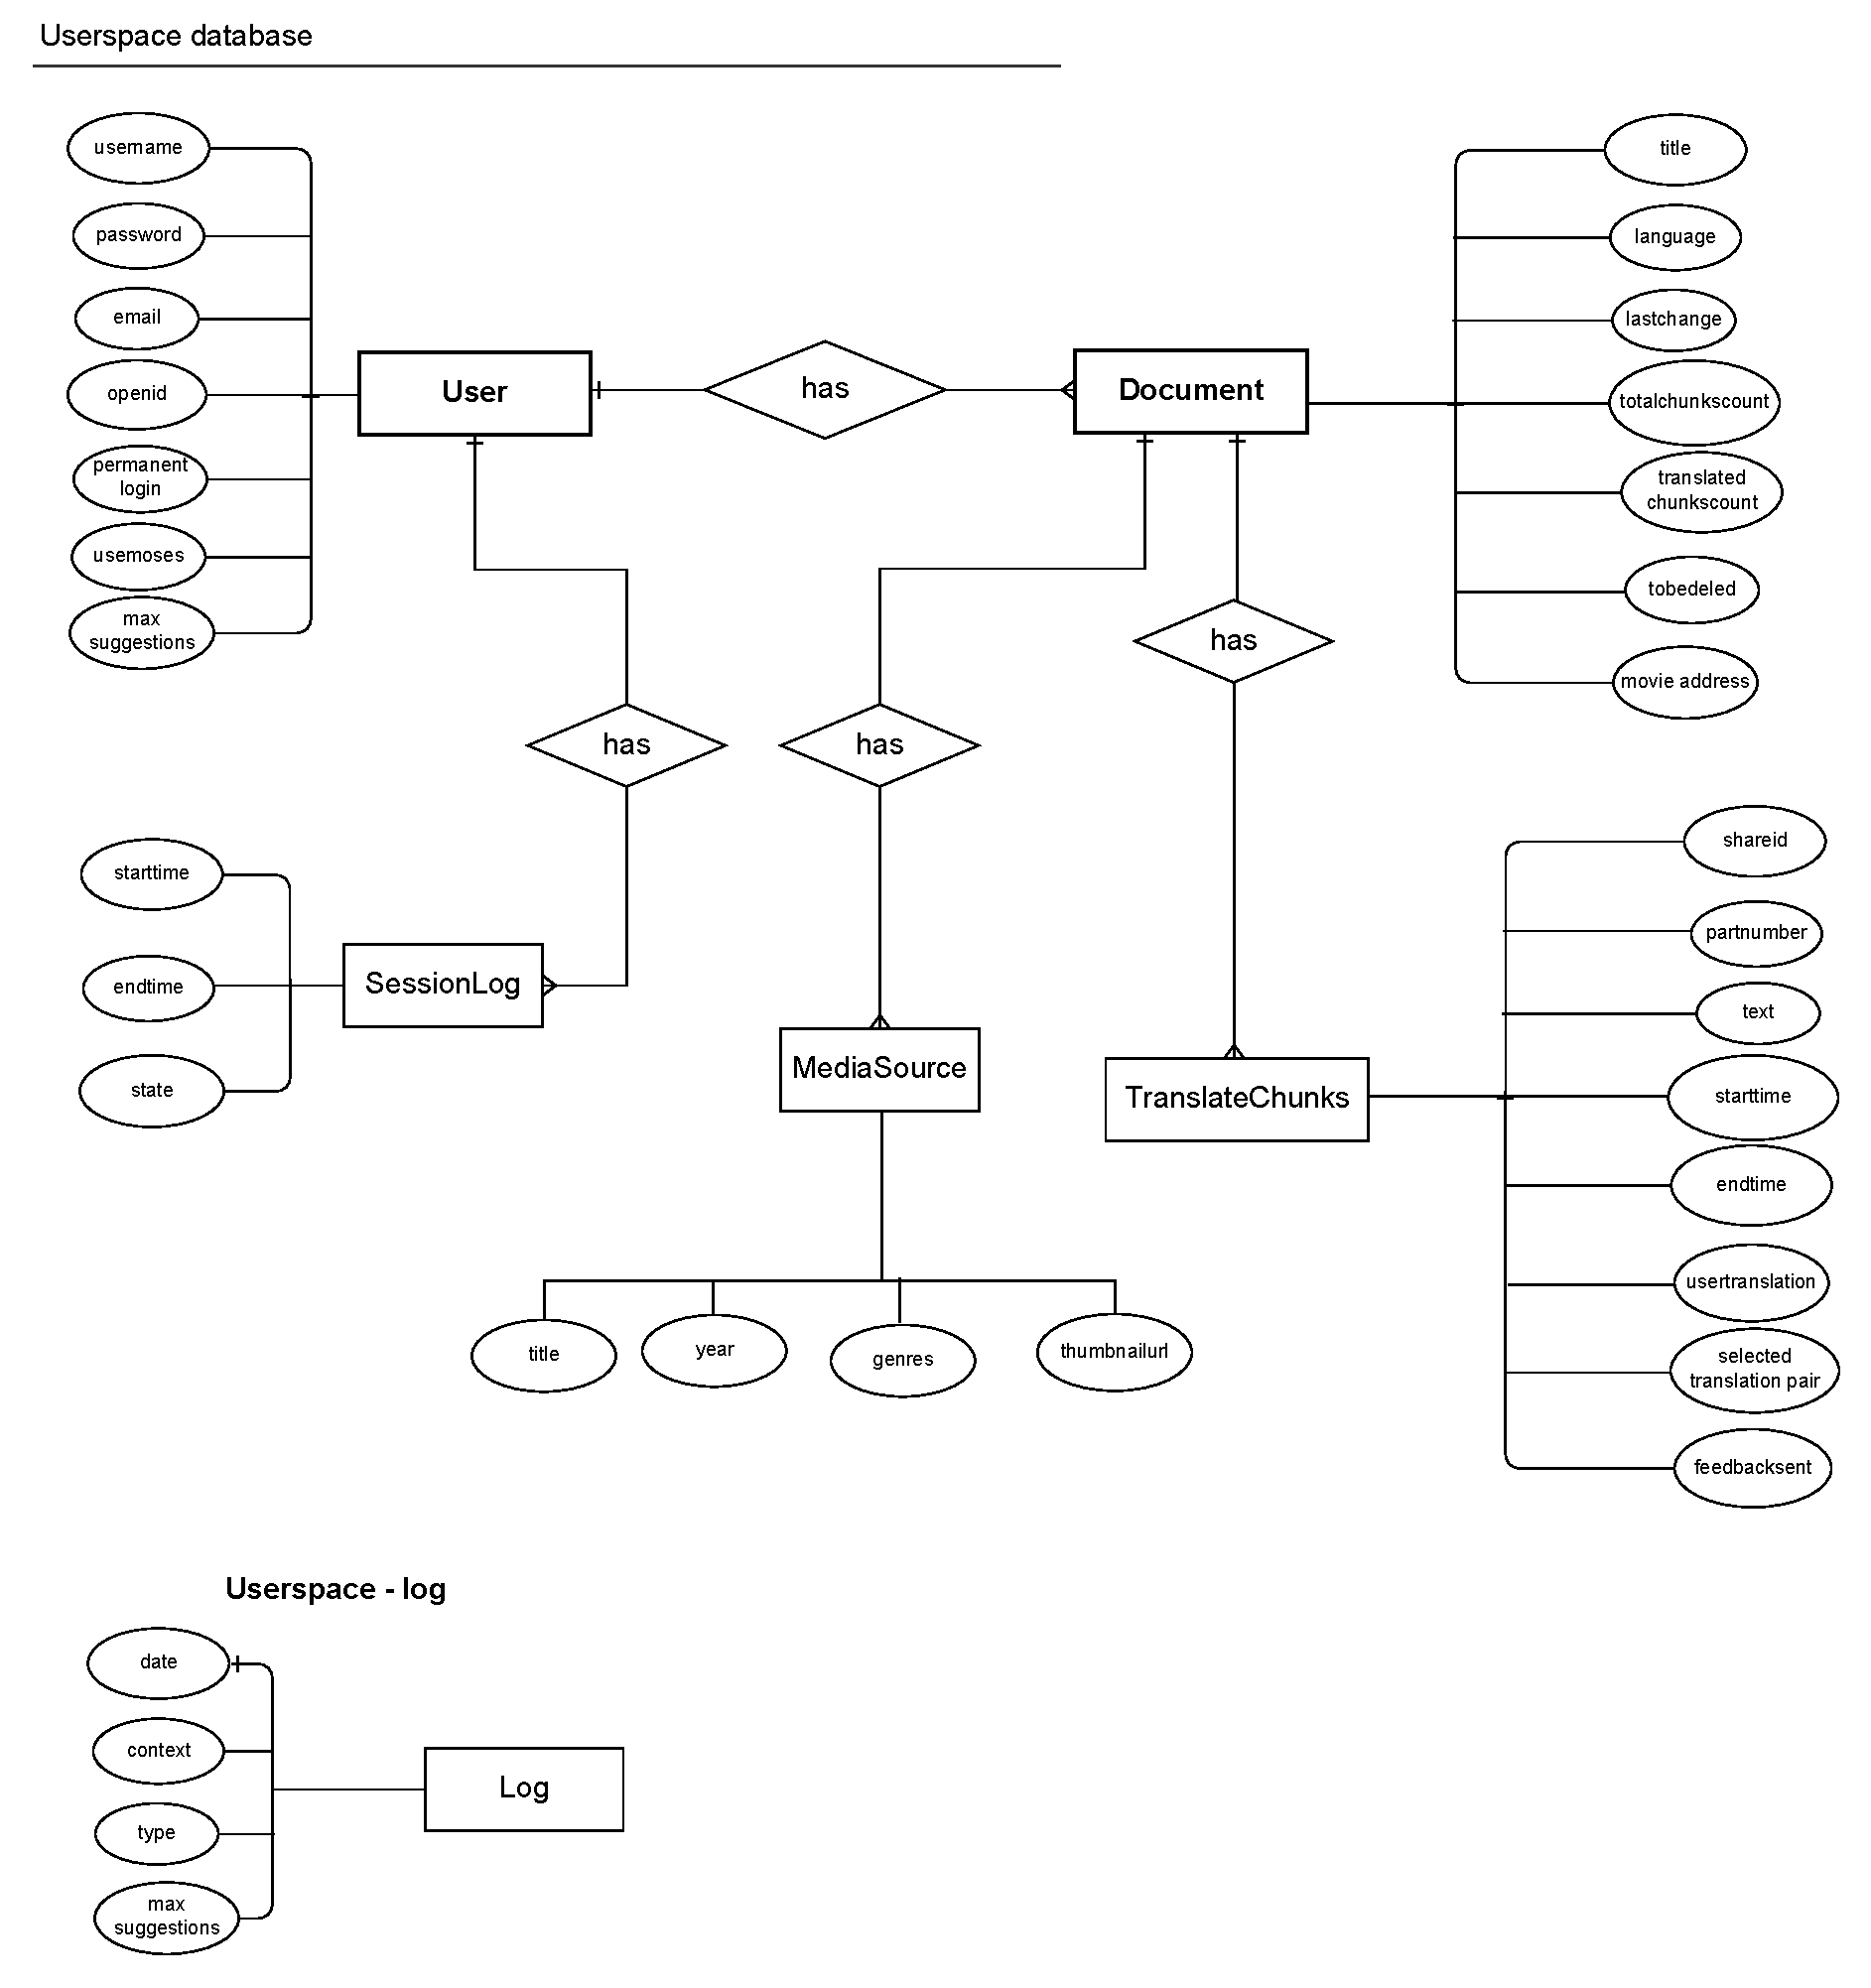
\includegraphics[scale=0.5]{figures/userspacedb.pdf}
\end{center}
\caption{EM diagram of the database used by the User Space}
\label{fig:em_of_us}
\end{figure}

\subsection{Providing Feedback to the Translation Memory}

In order to be able to provide feedback to the translation memory and take advantage of the translator work for improving the translation memory, the implementation of deleting a document and the selection of the media source should not be done synchronously. Handling this requirements is described in following paragraphs.

The User Space and the Translation Memory Core use the same database table for media sources (representing the movie or the TV show the subtitles are from). When the users create a document, they are required to enter the title of the movie about to be translated. After that, the {\it Freebase} service is queried for the movies and TV shows possibly having such title and a list of these matches is provided to the user to choose from. After the user chooses the media source, the media source object is sent back to the User Space. Then, a search in the database table for media sources is performed. If there is a record with the same title and the release year, its data (genres and thumbnails URL) are updated, if it is a completely new media source, it is saved to the table.

The reason for doing this is to not have duplicate media sources in the database and also the fact that the meta data of the movie should be available to the Data Import module when the feedback to the translation memory is provided.

Another issue to be mentioned here is the handling of document deletion. When the user clicks on the delete button in the interface, the document is marked to be deleted in the User Space and is removed from the list of documents owned by the user and from the list of documents that has been loaded during a session. From that time the document is not available for the user. After dealing with this a thread is run that deals with the translation results the document consists of. All the translation results that have already been used as feedback to the translation memory are deleted from the database. If the document is empty after this step, it is deleted too.

Providing the feedback itself is done by a static method of the {\tt USTranslsationResult} class. This method returns all the translation results what have not been used for feedback before ({\tt hasSentFeedback} flag set to false). The translation results are provided with a reference they belong to which allows to resolve the media source later. If the translation results are form a document that has been flagged as ready to be deleted, both the translation results and the document are deleted. Otherwise, the flag informing about having provided the feedback is set.

\section{Exporting Subtitle Files}
\label{sec:export}

Users can export the files in both .srt and .sub format.

Exporting the files is a straightforward task -- we just go through the chunks, maybe connect them to subtitle items if they have the same time, and save their contents.

However, there is a problem with the formats. While .srt format uses time information, .sub format uses frames. For transfering between them, you have to know the FPS (frames per second) of the actual movie file. FPS varies across files (it is usually between 23 and 50, depending on the source of the movie file).

Right now, we ask the user for FPS when exporting. Another solution would be to read the FPS from video file, loaded through the player (more about the player in ???), since VLC plug-in can read the FPS using javascript; we didn't implement that due to time constraints.

Another small issue with exporting is that we want to make the srt file downloadable. We cannot do that only using GWT and RPC, since GWT works through javascript, which cannot produce files to download. So instead we run a separate servlet, whose only responsibility is to produce .srt files. This servlet named \texttt{SubtitleDownloadServlet} is created at the start of the program, has a \texttt{FilmTitBackendServer} reference, and gets document ID and session ID through standard GET request.

We can export three different type of file:
\begin{itemize}
    \item file with only the translated chunks, completely omitting the untranslated ones,
    \item file with the translated chunks, with the source chunks at places where nothing is translated,
    \item file with only the source chunks.
\end{itemize}
All three types in either .sub or .srt format. We also export to .txt, which is just the text of the subtitles without any time information.